% !TEX root = ../../../Lazcorreta.Tesis.tex
% \ABIERTO%
En esta sección nos vamos a detener en la obtención de las \ars, concretamente en la función $genrules()$ que encuentra las reglas que verifican nuestros \itemsets frecuentes. Aparentemente es la parte más rápida del algoritmo \apriori. El algoritmo original propuesto por~\citet{AgrawalSrikant-FastAlgorithmsForMiningAssociationRules-1994} se muestra en el listado~\ref{alg:apriori-genrules}. $genrules()$ recibe como parámetros dos \kitemsets, el primero es siempre $l_k$ y el segundo es un subconjunto de $l_k$, del que se extraerán los \antecedentes de las \emph{reglas derivadas} de $l_k$. En cada llamada a $genrules()$ se obtiene la \confianza de una regla del tipo $a_m \Rightarrow c_i$, donde $c_i = l_k - a_m$, lo que supone dos llamadas a la función \soporte, función que ha de recorrer \aprioriL hasta el nivel determinado por el número de ítems del \kitemset que recibe como parámetro: $k + (k - m)$ búsquedas.





~\citeauthor{AgrawalSrikant-FastAlgorithmsForMiningAssociationRules-1994} observaron la siguiente característica:

\selectlanguage{english}
\begin{quote}%\em
We showed earlier that if $a \Rightarrow (l - a)$ does not hold, neither does $\tilde{a} \Rightarrow (l - \tilde{a})$ for any $\tilde{a} \subset a$. By rewriting, it follows that for a rule $(l - c) \Rightarrow c$ to hold, all rules of the form $(l - \tilde{c}) \Rightarrow \tilde{c}$ must also hold, where $\tilde{c}$ is a non-empty subset of $c$. For example, if the rule AB $\Rightarrow$ CD holds, then the rules ABC $\Rightarrow$ D and ABD $\Rightarrow$ C must also hold.
\end{quote}
\selectlanguage{spanish}

Tras lo cual proponen un segundo método más rápido cuando $minConf$ es grande: si detectamos que conf(ABC $\Rightarrow$ D) $< minConf$ ya sabemos que no es necesario comprobar las reglas AB $\Rightarrow$ CD, AC $\Rightarrow$ BD, BC $\Rightarrow$ AD, A $\Rightarrow$ BCD, B $\Rightarrow$ ACD, C $\Rightarrow$ ABD.

En nuestro estudio, en que queremos detectar reglas sin altas \confianzas, esto no es un adelanto si no una comprobación más que ralentizaría la ejecución del algoritmo.

Podemos mejorar notablemente el rendimiento del algoritmo analizando las características de las reglas que genera. El siguiente ejemplo ilustra nuestras observaciones al respecto.

%TODO: Utilizar un listing si pongo muchos más ejemplos
\begin{quote}
\textbf{Ejemplo}\\
Sea el $k$-itemset $l_k = \{1, 2, 3, 4, 5, 6\}$.
\begin{enumerate}
    \item La ejecución de $genrules(l_k, l_k)$ realizará una llamada recursiva a $genrules(l_k, \{1, 2, 3, 4, 5\})$ y ésta realiza una llamada a $genrules(l_k, \{1, 2, 3, 4\})$, entre otras.
    \item Posteriormente, la llamada inicial a $genrules(l_k, l_k)$ realizará una llamada a $genrules(l_k, \{1, 2, 3, 4, 6\})$  y ésta llamará de nuevo a $genrules(l_k, \{1, 2, 3, 4\})$, entre otras.
\end{enumerate}
En consecuencia, se llama a $genrules(l_k, \{1, 2, 3, 4\})$ dos veces, lo que generará duplicados de todas las llamadas hechas con los subconjuntos de $\{1, 2, 3, 4\}$ como segundo parámetro. Esto genera un gran número de búsquedas y cálculos repetidos, exponencial en función de $k$, que no aportan nada al estudio pues se trata de cálculos ya realizados y convenientemente almacenados.
\end{quote}

Esta característica hace aún más ineficiente el algoritmo original si recordamos el modo en que se almacena el \dataset de \itemsets frecuentes, \aprioriL, ya que para buscar el \soporte de un \kitemset hemos de recorrer \aprioriL desde su raíz buscando cada uno de los ítems que forman $l_k$. Si hacer una búsqueda ya es costoso por tener que hacer $k$ búsquedas individuales, repetirla cuando ya se ha hecho es un desperdicio de recursos.

% \afterpage{\clearpage}
\lstinputlisting[label=alg:apriori-genrules-modificado,
                 caption={Función $genrules()$ modificada},
                 float=htb,
                 basicstyle=\scriptsize]
                 {./contenido/arm/codigo/funAprioriGenrulesModificado}

El listado~\ref{alg:apriori-genrules-modificado} presenta nuestra propuesta, una modificación de la función $genrules()$ en la que hemos respetado la numeración del pseudocódigo original (véase el listado~\ref{alg:apriori-genrules}) para que sea más fácil identificar los cambios que introdujimos.

El primer cambio consiste en añadir como parámetro de $genrules()$ el \soporte de $l_k$. Con ello evitamos numerosas llamadas a la función $soporte()$ aprovechando el momento en que se ejecuta $genrules()$. No se hace ninguna llamada a $soporte(l_k$) pues al procesar cada \kitemset de \aprioriL ya lo tenemos localizado y podemos consultar directamente su \soporte en lugar de buscarlo, ahorrando las múltiples llamadas recursivas que hace el algoritmo original.

El cambio más relevante es el uso de la variable estática \texttt{a\_m\_processed} y su inicialización cada vez que entramos en un nivel nuevo de \aprioriL. En el bucle sólo hay que comprobar si el \itemset ya ha sido utilizado, si lo ha sido lo ignoramos y trabajamos con el siguiente \itemset, si no lo ha sido se anota como utilizado y se sigue el flujo normal del algoritmo original. Se utilizan pocos recursos para guardar este vector en memoria ya que estamos centrados en un único \kitemset y \texttt{a\_m\_processed} contendrá únicamente sus subconjuntos.









Para probar la eficiencia de nuestra propuesta frente a la propuesta original aplicamos ambos algoritmos con diferentes \soportes y \confianzas mínimos sobre los almacenes de transacciones \texttt{foodmart} y \texttt{T40I10D100K} contando el número de reglas que se analizan con cada uno de los métodos y el número de reglas que contiene cada almacén \D en esas condiciones.% También anotamos el tiempo empleado en cada una de las ejecuciones.

Las tablas \ref{tab:foodmart} y \ref{tab:T40I10D100K} muestran los resultados obtenidos en la ejecución de ambos algoritmos. En las columnas bajo el epígrafe "`analizadas"' se indica el número de reglas analizadas con cada método y entre paréntesis la relación entre este valor y las reglas finalmente encontradas. También se muestra el tiempo de ejecución en cada una de las situaciones tratadas para constatar que la reducción de cálculos influye en el tiempo necesario para llevarlas a cabo.

\begin{table}[htb]
   \begin{center}
   \scriptsize
      \begin{tabular}{cccccc} \hline
                      &          &           & \multicolumn{3}{c}{reglas} \\ \cline{4-6}
                      &          &           & \multicolumn{2}{c}{analizadas} & encontradas \\ \cline{4-5}
         fichero      & $minSup$ & $minConf$ & original    & modificado & \\ \cline{1-1}\cline{2-2}\cline{3-3} \cline{4-4}\cline{5-5} \cline{6-6}
         foodmart     & 0.005\%  & 90\%      & 905\,498    & 757\,085   & 137\,917 \\
         (Cálculos)   &          &           & (656.6\%)   & (548.9\%)  & \\
         {Tiempo}&          &           & {3.6 sg}      & {3.1 sg}     & \\
                      &          & 75\%      & 932\,697    & 768\,962   & 149\,711 \\
                      &          &           & (623.0\%)   & (513.6\%)  & \\
                      &          &           & {3.8 sg}      & {3.2 sg}     & \\
                      &          & 50\%      & 1\,304\,152 & 865\,132   & 290\,441 \\
                      &          &           & (449.0\%)   & (297.9\%)  & \\
                      &          &           & {5.7 sg}      & {4.5 sg}     & \\
                      &          & 25\%      & 1\,437\,624 & 870\,460   & 338\,221 \\
                      &          &           & (425.1\%)   & (257.4\%)  & \\
                      &          &           & {6.3 sg}      & {4.8 sg}     & \\
                      &          & 5\%       & 1\,442\,456 & 870\,464   & 340\,375 \\
                      &          &           & (423.8\%)   & (255.7\%)  & \\
                      &          &           & {6.3 sg}      & {4.8 sg}     & \\
                      &          & 1\%       & 1\,442\,456 & 870\,464   & 868\,427 \\
                      &          &           & (166.1\%)   & (100.2\%)  & \\
                      &          &           & {10.8 sg}     & {6.9 sg}     & \\
                      &          & 0\%       & 1\,442\,456 & 870\,464   & 870\,464 \\
                      &          &           & (165.7\%)   & (100\%)    & \\
                      &          &           & {10.7 sg}     & {7.0 sg}     & \\ \hline
      \end{tabular}
   \end{center}

   % \caption[Algoritmo modificado vs original (foodmart)]{Reglas analizadas y encontradas (foodmart)}
   \caption{Reglas analizadas y encontradas (foodmart)}
   \label{tab:foodmart}
\end{table}

La figura~\ref{fig:2-3-1-genrulesFoodmart} ilustra los resultados obtenidos al analizar el almacén \texttt{foodmart}. Es fácil observar en estas gráficas que la reducción de cálculos realizados y de tiempo es mayor cuanto menor es la \confianza mínima utilizada.

\begin{figure}[hbt]
  \centering
  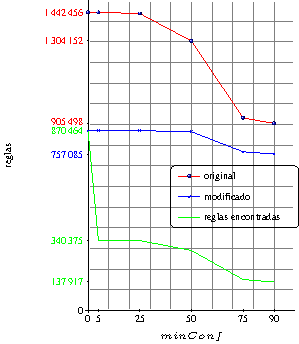
\includegraphics[width=.35\textwidth]{2-2-numReglas-foodmart.pdf}
  \hspace{.1\textwidth}
  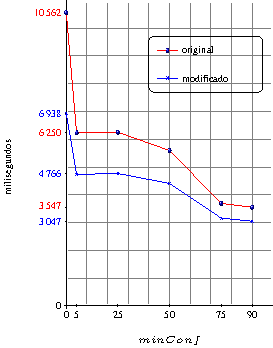
\includegraphics[width=.31\textwidth]{2-2-tiempo-foodmart.pdf}
  % \caption{Reglas analizadas (foodmart, $minSup = 0.005\%$)}
	\caption[\texttt{genrules()} original vs. nuestra modificación]{\footnotesize \texttt{genrules()} original vs. nuestra modificación (\texttt{foodmart}, $minSup=0.005\%$)}
	\label{fig:2-3-1-genrulesFoodmart}
\end{figure}


% \begin{wrapfigure}{o}{0.45\textwidth}
%   \centering
%   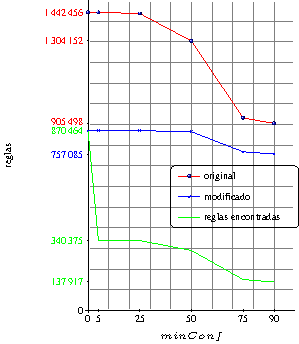
\includegraphics[width=.42\textwidth]{2-2-numReglas-foodmart.pdf}
%   % \caption{Reglas analizadas (foodmart, $minSup = 0.005\%$)}
%   \caption{\footnotesize Reglas analizadas (foodmart)}
%   \label{fig:2-3-1-numReglasFoodmart}
% \end{wrapfigure}
La primera observación a destacar de estos resultados es que la eficiencia de nuestro método depende de su implementación. Cuando no se impone un umbral de \confianza ($minConf = 0\%$) estamos obligando al algoritmo a mostrar todas las reglas existentes. En estas condiciones nuestro método analiza únicamente las reglas que contiene el almacén \D mientras que el método original analiza un 65.7\% más de las reglas encontradas en el análisis de \texttt{foodmart} y hasta un 13\,016.0\% más en el peor de los casos estudiados, al analizar \texttt{T40I10D100K} con \soporte mínimo del 0.5\%.




%TODO: Falta un valor, minSup = 0.1\%, minConf = 50\%
\begin{table}[htb]
   \scriptsize
   \begin{center}
      \begin{tabular}{cccccc} \hline
                     &          &        & \multicolumn{3}{c}{reglas} \\ \cline{4-6}
                     &          &        & \multicolumn{2}{c}{analizadas} & encontradas \\ \cline{4-5}
         fichero     & $minSup$ & $minConf$ & original   & modificado  & \\ \cline{1-1}\cline{2-2}\cline{3-3} \cline{4-4}\cline{5-5} \cline{6-6}
         T40I10D100K & 5\%      & 50\%   & 30            & 30          & 0 \\                      %Comprobado
         (Cálculos)  &          &        & ()            & ()          & \\
         Tiempo      &          &        & 0 msg         & 0 msg       & \\
                     & 1\%      & 50\%   & 5\,193\,340   & 398\,818    & 290\,273 \\
                     &          &        & (1\,789.1\%)  & (137.4\%)   & \\
                     &          &        & 30.3 sg       & 4.1 sg      & \\
                     &          & 0\%    & 5\,912\,979   & 401\,096    & 401\,096 \\
                     &          &        & (1\,474.2\%)  & (100\%)     & \\
                     &          &        & 30.3 sg       & 4.1 sg      & \\
                     & 0.5\%    & 50\%   & 606\,619\,662 & 6\,302\,454 & 4\,927\,893 \\
                     &          &        & (12\,309.9\%) & (127.9\%)   & \\
                     &          &        & 4\,772.7 sg   & 91.2 sg     & \\
                     &          & 0\%    & 846\,495\,481 & 6\,453\,924 & 6\,453\,924 \\
                     &          &        & (13\,116.0\%) & (100\%)     & \\
                     &          &        & 14\,266.6 sg  & 106.1 sg    & \\ \hline
      \end{tabular}
   \end{center}
   \caption{Reglas analizadas y encontradas (T40I10D100K)}
   \label{tab:T40I10D100K}
\end{table}



Al incrementar la \confianza mínima se analizan más reglas de las que finalmente serán aceptadas ya que muchas de ellas no superarán el umbral fijado. A pesar de que se acercan los valores obtenidos usando ambos algoritmos siempre se produce un gran ahorro al utilizar nuestra propuesta.

% En el almacén \texttt{T40I10D100K} peor de los casos analizamos con nuestra propuesta un 448\% más de las reglas existentes, correspondiendo a las reglas que no superan el umbral de \confianza fijado. El algoritmo original analiza en este caso un 556\% más de reglas.

Todo esto también se refleja en el tiempo de ejecución, notablemente inferior en todas las pruebas realizadas para el algoritmo modificado, hasta el extremo de tardar menos de 2 minutos en una ejecución en que el algoritmo original empleó más de 237 minutos (\texttt{T40I10D100K} con $minSup = 0.5\%$ y $minConf = 0\%$). Si aplicamos nuestra propuesta a las transacciones realizadas por un único usuario serán aún menores los tiempos, consiguiendo resultados en tiempo real para alimentar un \srw.





